\documentclass[12pt]{beamer}
\usetheme{madrid}
\setbeamertemplate{navigation symbols}{}

% ── Pacotes ─────────────────────────────────────────────────
\usepackage[brazil]{babel}
\usepackage[utf8]{inputenc}
\usepackage[T1]{fontenc}
\usepackage{lmodern}
\usepackage{amsmath, amssymb, amsthm}
\usepackage{graphicx}
\usepackage{booktabs}
\usepackage{xcolor}
\usepackage{tikz}
\usetikzlibrary{arrows.meta, positioning, shapes.geometric}
\usepackage{listings}
\usepackage{hyperref}
\usepackage{multicol}
\usepackage{svg}

\graphicspath{ {./figuras/} }

\AtBeginSection[]
{
  \begin{frame}
    \frametitle{Sumário}
    \tableofcontents[currentsection]
  \end{frame}
}

% ── Metadados ───────────────────────────────────────────────
\title{Animação Física Simplificada em Web}
\subtitle{Trabalho de Conclusão de Curso}
\author[Diego V. S. de Matos]{Diego Vasconcelos Schardosim de Matos}
\institute[UFRJ]{Universidade Federal do Rio de Janeiro\\
  Instituto de Computação}
\date{\today}
\logo{
\includegraphics[height=1cm]{ufrj-vertical-cor-rgb-telas.png}}

% ============================================================
\begin{document}
% ============================================================

% ── Slide de título ─────────────────────────────────────────
\maketitle

% ── Sumário ─────────────────────────────────────────────────
% \begin{frame}{Sumário}
%   \tableofcontents[hideallsubsections]
% \end{frame}

% ============================================================
\section{Introdução}
% ============================================================

\begin{frame}{Motivação}
    \begin{itemize}
        \item Aplicações interativas exigem realismo visual
              \textbf{e} alto desempenho 
        \item Aplicabilidade em jogos, simulações educacionais, robótica
        \item Animação física une dois domínios:
          \begin{itemize}
            \item \textbf{Geometria} — detecção e cálculo de contatos
            \item \textbf{Física} — evolução dinâmica dos corpos
          \end{itemize}
        \item Método de Jakobsen~\cite{jakobsen2001advanced}: esquema
              simplificado sem torques, matrizes de orientação nem
              tensores de inércia explícitos — mas com lacunas a explorar
      \end{itemize}
\end{frame}

\begin{frame}{Pipeline de animação física}
    \begin{enumerate}
        \item Definição dos corpos
        \item Integração numérica
        \item Detecção de colisões
        \item Resposta às colisões
        \item Renderização (WebGL)
    \end{enumerate}
    
    \vspace{0.3cm}
    \begin{alertblock}{}
        \footnotesize
        Motores de referência: Havok, PhysX, Bullet, Box2D. Todos inspiram a proposta Web deste trabalho.
    \end{alertblock}
\end{frame}

% ── ── ── ── ── ── ── ── ── ── ── ── ── ── ── ── ── ── ── ──
\begin{frame}{Objetivos}
  Desenvolver um protótipo de animação física 2D para a Web,
  inspirado no método de Jakobsen, com detecção e resposta a colisões.

  \vspace{0.4cm}
  \textbf{Objetivos Específicos:}
  \begin{enumerate}
    \item Revisar os principais conceitos de animação baseada em
          física e integração numérica
    \item Implementar algoritmos de detecção e resposta a colisão
    \item Desenvolver simulação física baseada em partículas e
          restrições pelo método de Jakobsen~\cite{jakobsen2001advanced}
    \item Aplicar técnicas de otimização para garantir desempenho em tempo real
    \item Avaliar o desempenho e a estabilidade do sistema em
          diferentes cenários (\textit{benchmarks})
  \end{enumerate}
\end{frame}

% ============================================================
\section{Animação Baseada em Física}
% ============================================================

\begin{frame}{Conceitos}
  \begin{columns}[T]
    \column{0.50\textwidth}
      \begin{block}{\textit{Keyframe} vs.\ Baseada em Física}
        \begin{itemize}
          \item \textbf{\textit{Keyframe}:} animador define manualmente
                posições e rotações ao longo do tempo
          \item \textbf{Física:} comportamento \textit{emerge} de forças,
                restrições e interações entre corpos
        \end{itemize}
      \end{block}
    \column{0.47\textwidth}
      \textbf{Ciclo de simulação:}
      \begin{enumerate}
        \item Coleta e soma de forças\\(gravidade, vento, atrito\ldots)
        \item Integração temporal das\\equações de movimento
        \item Detecção e resposta\\a colisões
        \item Atualização de posições\\e renderização
      \end{enumerate}
  \end{columns}

    \begin{alertblock}{Foco: verossimilhança visual}
        O objetivo \textbf{não} é precisão científica, mas
        \textbf{plausibilidade} — transmitir sensação convincente de
        peso, inércia e colisão ao usuário.
    \end{alertblock}
\end{frame}

% ── ── ── ── ── ── ── ── ── ── ── ── ── ── ── ── ── ── ── ──
\begin{frame}{Representação dos Corpos}
  \begin{columns}[T]
    \column{0.48\textwidth}
      \begin{block}{Corpo Rígido}
        Forma e volume \textbf{invariáveis}
        % . Representado por grandezas globais:
        % \begin{itemize}
        %   \item Posição $\vec{p}$ (centro de massa)
        %   \item Orientação $R$ (matriz ou quatérnio)
        %   \item Velocidades linear $\vec{v}$ e angular $\vec{\omega}$
        %   \item Massa $m$ e tensor de inércia $I$
        % \end{itemize}
      \end{block}
    \column{0.48\textwidth}
      \begin{block}{Corpo Deformável}
        Forma varia sob forças externas. 
        % Modelado por sistemas de
        % \textbf{partículas + molas} (\textit{massa-mola}):
        % \[
        %   \vec{F}_{\text{el}} = -k_s\bigl(|\vec{x}_i - \vec{x}_j| - L_0\bigr)
        %     \frac{\vec{x}_i - \vec{x}_j}{|\vec{x}_i - \vec{x}_j|}
        % \]
        % \[
        %   \vec{F}_{\text{am}} = -k_d\,(\vec{v}_i - \vec{v}_j)
        %     \frac{\vec{x}_i - \vec{x}_j}{|\vec{x}_i - \vec{x}_j|}
        % \]
      \end{block}
  \end{columns}
\end{frame}

% ── ── ── ── ── ── ── ── ── ── ── ── ── ── ── ── ── ── ── ──
\begin{frame}{Método de Integração Numérica}
  Jakobsen~\cite{jakobsen2001advanced} adota um método de segunda ordem que \textbf{não armazena velocidade explicitamente}. O integrador de Verlet calcula a nova posição a partir das posições atual e anterior:
  \[
    \vec{x}_{t+\Delta t} = 2\,\vec{x}_t - \vec{x}_{t-\Delta t}
      + \vec{a}_t\,\Delta t^2
  \]

  \vfill
  \begin{columns}
    \column{0.5\textwidth}
      Velocidade derivada implicitamente quando necessária:
      \[
        \vec{v}_t \approx
          \frac{\vec{x}_{t+\Delta t} - \vec{x}_{t-\Delta t}}{2\,\Delta t}
      \]
    
    \column{0.5\textwidth}
      Vantagens:
      \begin{itemize}
          \item Estável sob restrições geométricas
          \item Menos armazenamento por partícula
      \end{itemize}
  \end{columns}
\end{frame}

% ── ── ── ── ── ── ── ── ── ── ── ── ── ── ── ── ── ── ── ──
\begin{frame}{Restrições Geométricas — Jakobsen}
  \begin{block}{Restrição de distância (linear)}
    Mantém distância fixa $d$ entre partículas $i$ e $j$ a todo instante:
    \[
      |\vec{x}_i - \vec{x}_j| = d
      \]
  \end{block}
  Após cada passo de integração, as partículas são \textbf{projetadas}
  de volta para a configuração válida.
\end{frame}

\begin{frame}
  \begin{figure}[htb]
    \centering
    \includesvg[width=\textwidth]{restricao-linear}
    \caption{A distância atual entre as partículas $p_1$ e $p_2$ está inválida e deve ser corrigida por projeção. Fonte: Autor.}
      \label{fig:correcao}
  \end{figure}
\end{frame}

% ── ── ── ── ── ── ── ── ── ── ── ── ── ── ── ── ── ── ── ──
\begin{frame}{Resolvendo Restrições Concorrentes por Relaxamento}
  \begin{block}{Método iterativo de Jakobsen (Gauss-Seidel)}
    Restrições são resolvidas \textbf{sequencialmente} e repetidas até
    convergência, geralmente de 3 a 5 iterações são suficientes.
  \end{block}
  
  \begin{columns}
    \column{0.5\textwidth}
      \textbf{Algoritmo de relaxamento para restrição linear:}
      \[
        \vec{\delta} = \vec{x}_2 - \vec{x}_1, \qquad
        c = \frac{\|\vec{\delta}\| - d}{\|\vec{\delta}\|}
      \]
      \[
        \vec{x}_1 \leftarrow \vec{x}_1 - \epsilon\,\vec{\delta}\,c, \qquad
        \vec{x}_2 \leftarrow \vec{x}_2 + \epsilon\,\vec{\delta}\,c
      \]

    \column{0.5\textwidth}
      \begin{itemize}
        \item $\epsilon = 1$: partículas movidas \textit{imediatamente}
                para a posição correta (haste rígida)
        \item $\epsilon < 1$: convergência gradual (mola rígida)
        \item Mais iterações $\Rightarrow$ animação mais rígida
                visualmente
      \end{itemize}
  \end{columns}

\end{frame}

% ── ── ── ── ── ── ── ── ── ── ── ── ── ── ── ── ── ── ── ──
\begin{frame}{Estrutura Topológica para Tecidos}
  Partículas organizadas em grade; estabilidade depende dos tipos de
  conexão:

  \begin{enumerate}
    \item \textbf{Restrições estruturais} — vizinhos diretos (horizontal e
          vertical); resistem à tração e compressão básicas
    \item \textbf{Restrições de cisalhamento} — vizinhos diagonais; impedem
          distorção e deslizamento da malha
    \item \textbf{Restrições de flexão} — vizinhos alternados (pulam um
          nó); resistem à dobra e conferem rigidez à curvatura
  \end{enumerate}

  \begin{tikzpicture}
    \foreach \x in {0,1,2} \foreach \y in {0,1,2}
      \filldraw[black] (\x,\y) circle (2.5pt);
    \foreach \x in {0,1} \foreach \y in {0,1,2}
      \draw[black, thick] (\x,\y) -- (\x+1,\y);
    \foreach \x in {0,1,2} \foreach \y in {0,1}
      \draw[black, thick] (\x,\y) -- (\x,\y+1);
    \foreach \x in {0,1} \foreach \y in {0,1} {
      \draw[gray, dashed] (\x,\y) -- (\x+1,\y+1);
      \draw[gray, dashed] (\x+1,\y) -- (\x,\y+1);
    }
    \draw[black, thick] (3.2,1.8) -- (3.8,1.8)
      node[right, font=\tiny] {Estrut.};
    \draw[gray, dashed] (3.2,1.3) -- (3.8,1.3)
      node[right, font=\tiny] {Cisalh.};
  \end{tikzpicture}
\end{frame}

% ============================================================
\section{Detecção de Colisões}
% ============================================================
 
% ── Slide 1: Visão geral ────────────────────────────────────
\begin{frame}{Detecção de Colisões — Visão Geral}
  \begin{block}{Objetivo}
    Identificar quando dois objetos entram em contato e fornecer
    informações geométricas (vetor de penetração, normal) para a etapa
    de resposta física.
  \end{block}
 
    Dois algoritmos estudados e implementados, ambos eficientes para
    objetos \textbf{convexos}:
    \begin{itemize}
        \item \textbf{SAT} — Teorema do Eixo Separador
        \item \textbf{GJK} — Gilbert-Johnson-Keerthi
    \end{itemize}
\end{frame}
 
% ── Slide 2: SAT ────────────────────────────────────────────
\begin{frame}{Teorema do Eixo Separador (SAT)}
  \begin{block}{Teorema}
    Dois polígonos convexos $A$ e $B$ \textbf{não se intersectam} se, e
    somente se, existe um hiperplano separador $P$ tal que $A$ está de
    um lado de $P$ e $B$ está do outro \cite{ericson2004real}.
  \end{block}
  
  \textbf{Ideia prática:} testar as normais das arestas de ambos os
  polígonos como eixos candidatos. Para cada eixo $\hat{n}$:
  \[
    \text{Sobreposição} \iff
    \max_A \geq \min_B \;\wedge\; \max_B \geq \min_A
  \]
  Se \textit{qualquer} eixo separar as projeções, os objetos \textbf{não colidem} e o algoritmo encerra imediatamente.
  
\end{frame}

\begin{frame}
  \begin{figure}[htb]
    \centering
    \includesvg[width=0.5\linewidth]{eixo-separador}
    \caption{Aresta escolhida em amarelo, eixo separador perpendicular à face. Fonte: Autor}
    \label{fig:eixo-separador}
  \end{figure}
\end{frame}
 
% ── Slide 3: GJK — Diferença de Minkowski ───────────────────
\begin{frame}{Algoritmo GJK - Fundamentos}
  \begin{block}{Soma de Minkowski}
    Seja dois conjuntos convexos $A$ e $B$ em $\mathbb{R}^n$. A soma de Minkowski é definida como:
    $$A + B = \{\,\vec{x} + \vec{y} \mid \vec{x} \in A,\; \vec{y} \in B\,\},$$
    onde $\vec x$ e $\vec y$ representam vetores posição associados a pontos pertencentes aos conjuntos A e B, respectivamente.
  \end{block}
\end{frame}

\begin{frame}{Algoritmo GJK - Fundamentos}
  \begin{figure}[htb]
    \centering
    \includesvg[width=0.7\linewidth]{soma-minkowski}
    \caption{Soma de Minkowski, entre os conjuntos A e B. Fonte: Autor.}
    \label{fig:soma-minkowski}
  \end{figure}
\end{frame}

\begin{frame}{Algoritmo GJK — Fundamentos}
  \begin{block}{Ideia central}
    Dois objetos $A$ e $B$ se intersectam se, e somente se, a
    \textbf{diferença de Minkowski} (CSO) contém a origem:
    \[
      A - B = \{\,\vec{x} - \vec{y} \mid \vec{x} \in A,\; \vec{y} \in B\,\}
    \]
    \[
      d(A,B) = \min_{c \in \text{CSO}} \|\,c\,\|
    \]
  \end{block}

  O CSO \textbf{não é calculado explicitamente}. Em vez disso,
  amostras são obtidas sob demanda usando uma \textbf{função suporte}.
  
\end{frame}

\begin{frame}{Algoritmo GJK - Fundamentos}
  Seja A um conjunto qualquer, o suporte de A na direção de $\vec d$ retorna o ponto que pertence a superfície de A mais distante da origem na direção $\vec d$, esse ponto é chamado de ponto de suporte
  \begin{align*}
    S_A(\vec d) &= \arg\max_{\vec a \in A} (\vec d \cdot \vec a), \\
    S_{A+B} (\vec d) &= S_A (\vec d) + S_B (\vec d), \\
    S_{-A} (\vec d) &= -S_A (-\vec d).
  \end{align*}

  Dessa forma, seja $D$ a diferença de Minkowski de dois objetos convexos $A$ e $B$, o suporte de $D$ na direção $\vec d$ é a diferença dos suportes de $A$ e $B$: $S_{A-B} (\vec d) = S_A (\vec d) - S_B (-\vec d)$, como ilustrado pela Figura~\ref{fig:support_function}. 

\end{frame}
 
% ── Slide 4: GJK — Simplex e algoritmo ──────────────────────
\begin{frame}{Algoritmo GJK — Iteração sobre Simplices}
  \begin{columns}[T]
    \column{0.52\textwidth}
      O GJK constrói iterativamente \textbf{simplices} dentro do CSO,
      aproximando-se da origem:
      \begin{itemize}
        \item 0-simplex: ponto
        \item 1-simplex: segmento
        \item 2-simplex: triângulo (em 2D)
        \item 3-simplex: tetraedro (em 3D)
      \end{itemize}
    \column{0.45\textwidth}
      \begin{figure}[htb]
        \centering
        \includesvg[width=\textwidth]{simplex}
        % \caption{Da esquerda para direita 0-simplex, 1-simplex, 2-simplex e 3-simplex. Fonte: Autor.}
        \label{fig:simplex}
      \end{figure}
  \end{columns}
  
  A cada iteração, um novo ponto de suporte $\vec{s}$ é adicionado.
  Se $\vec{s} \cdot \vec{d} \leq 0$, a origem \textbf{não pertence}
  ao CSO, sem colisão.
\end{frame}
 
% ── Slide 5: Subalgoritmo de Ericson — 1-simplex ────────────
\begin{frame}{Subalgoritmo de Ericson — Caso 1-simplex}
  Segmento $RS$ divide o espaço em \textbf{três regiões}:
  região do vértice $R$, região do vértice $S$ e região da aresta
  $\vec{rs}$.
  % NOTA: Ericson usa o termo "regiões de Voronoi" de forma equivocada;
  % o correto é apenas "regiões", pois há dois sítios e duas regiões
  % de Voronoi, não três.
 
  \begin{columns}[T]
    \column{0.48\textwidth}
      \begin{itemize}
        \item Origem na \textbf{região de $R$}: descarta $S$,
              $\vec{d} = \vec{ro}$
        \item Origem na \textbf{região de $S$}: descarta $R$,
              $\vec{d} = \vec{so}$
        \item Origem na \textbf{região da aresta}: mantém $\{R,S\}$,
              $\vec{d} = (\vec{rs} \times \vec{ro}) \times \vec{rs}$
      \end{itemize}
      \vspace{0.2cm}
      Regiões de vértice estão além do limite do CSO $\Rightarrow$
      origem nessas regiões implica \textbf{sem colisão}.
    \column{0.48\textwidth}
      \begin{figure}[htb]
        \centering
        \includesvg[width=\textwidth]{gjk-ericson-1simplex.svg}
        % \caption{Divisão de regiões para o caso 1-simplex. Fonte: Adaptado de~\cite{muratori2016implementingGJK}.}
        \label{fig:gjk-ericson-1simplex}
      \end{figure}
  \end{columns}
\end{frame}
 
% ── Slide 6: Subalgoritmo de Ericson — 2-simplex ────────────
\begin{frame}{Subalgoritmo de Ericson — Caso 2-simplex}
  Triângulo $RST$ possui \textbf{7 regiões}, mas o histórico de
  construção elimina 4 delas. Verifica-se apenas: aresta $\vec{rs}$,
  aresta $\vec{rt}$ e interior do $\triangle RST$.
 
  \begin{columns}[T]
    \column{0.52\textwidth}
      Seja $\vec{n} = \vec{rs} \times \vec{rt}$:
      \begin{itemize}
        \item Se $(\vec{n} \times \vec{rs}) \cdot \vec{ro} > 0$
              $\Rightarrow$ origem na região de $\vec{rs}$:
              executar caso 1-simplex$(\{R,S\})$
        \item Se $(\vec{rt} \times \vec{n}) \cdot \vec{ro} > 0$
              $\Rightarrow$ origem na região de $\vec{rt}$:
              executar caso 1-simplex$(\{R,T\})$
        \item Caso contrário $\Rightarrow$ origem no interior
              do triângulo: \textbf{colisão detectada}
      \end{itemize}
    \column{0.45\textwidth}
      \begin{figure}[htb]
        \centering
        \includesvg[width=\linewidth]{gjk-ericson-2simplex.svg}
        % \caption{Regiões para o caso 2-simplex. Fonte: Adaptado de~\cite{muratori2016implementingGJK}.}
        \label{fig:gjk-ericson-2simplex}
      \end{figure}
  \end{columns}
\end{frame}

% ============================================================
\section{Resposta a Colisões}
% ============================================================
 
% ── Slide 1: Conceitos e métodos ────────────────────────────
\begin{frame}{Resposta a Colisões — Conceitos}
  \begin{block}{Duas operações principais}
    \begin{enumerate}
      \item \textbf{Correção de posição:} eliminar a interpenetração
      \item \textbf{Correção de velocidade:} evitar novo contato imediato
    \end{enumerate}
  \end{block}
 
  \vspace{0.3cm}
  \textbf{Principais abordagens na literatura:}
  \begin{itemize}
    \item \textbf{Método do Impulso} — aplica impulsos instantâneos que
          alteram velocidades preservando momento linear e angular
          (Havok, Bullet)
    \item \textbf{Método de Penalidades} — forças de repulsão
          proporcionais à penetração (modelo mola-amortecimento);
          simples, mas sensível a parâmetros de rigidez
    \item \textbf{Restrições + Lagrange} — formulação robusta; exige
          solução de sistemas lineares — oneroso em plataformas Web
    \item \textbf{Jakobsen (este trabalho)} — colisões tratadas como
          \textbf{restrições geométricas} corrigidas por posição,
          dentro do laço de relaxamento
  \end{itemize}
\end{frame}
 
% ── Slide 2: Manifold de colisão ────────────────────────────
\begin{frame}{Pontos de Contato e Manifold de Colisão}
  \begin{block}{Pontos de contato}
    Posições onde dois objetos se tocam. Obtidos a partir da
    geometria no instante em que se detecta a interpenetração.
    Podem ser um único ponto (vértice-face) ou múltiplos (face-face).
  \end{block}
  \vfill
  \begin{block}{Manifold de colisão}
    Estrutura que agrega os pontos de contato com:
    \begin{itemize}
      \item \textbf{Normal de colisão} $\hat{n}$ direção de
            separação entre os objetos
      \item \textbf{Profundidade de penetração} $d$ 
      \item Pontos envolvidos na colisão.
    \end{itemize}
  \end{block}
\end{frame}
 
% ── Slide 3: SAT com MTV ────────────────────────────────────
\begin{frame}{SAT com Cálculo do MTV}
  \begin{block}{Vetor de Translação Mínima (MTV)}
    Extensão do SAT: em vez de encerrar ao encontrar um eixo separador,
    \textbf{todos os eixos são testados}. O eixo com a
    \textbf{menor sobreposição} fornece a normal de contato $\hat{n}$ e
    a profundidade de penetração $\delta$.
  \end{block}

  Para cada aresta normal $\hat{n}$ de $A$ e $B$:
  \[
    \Delta = \text{sobreposição das projeções de } A \text{ e } B
  \]
  \begin{itemize}
    \item Se $\Delta \leq \epsilon$ $\Rightarrow$ \textbf{sem colisão},
          retorna imediatamente
    \item Se $\Delta < \delta_{\min}$ $\Rightarrow$ atualiza MTV:
          $\delta \leftarrow \Delta$,\; $\hat{n}_{\text{MTV}} \leftarrow \hat{n}$
  \end{itemize}
  Ao fim, $(\hat{n}_{\text{MTV}},\, \delta)$ descrevem a menor
  translação para separar os objetos.
\end{frame}
 
% ── Slide 4: EPA ────────────────────────────────────────────
\begin{frame}{Algoritmo de Expansão de Politopos (EPA)}
  \begin{block}{Motivação}
    O GJK detecta a colisão, mas não fornece $\hat{n}$ nem $\delta$.
    O EPA resolve o problema dual: encontrar o \textbf{MTV} a partir
    do simplex final do GJK.
  \end{block}
  \vspace{0.2cm}
  \textbf{Iteração:}
  \begin{enumerate}
    \item Selecionar a \textbf{aresta mais próxima} da origem
    \item $\vec{p}$: ponto mais próximo da origem na aresta
          ($\|\vec{p}\|$ = limite \textit{inferior} de $\delta$)
    \item $\vec{w} = S_{\text{CSO}}(\vec{p})$: novo vértice na
          fronteira do CSO
          ($\|\vec{w}\|$ = limite \textit{superior} de $\delta$)
    \item Subdividir a aresta em $\vec{w}$; repetir até
          $\|\vec{w}\| - \|\vec{p}\| < \epsilon$
  \end{enumerate}
  Retorna: normal $\hat{n}_e$ e profundidade $\delta$.
\end{frame}

\begin{frame}
  \begin{figure}[htb]
    \centering
    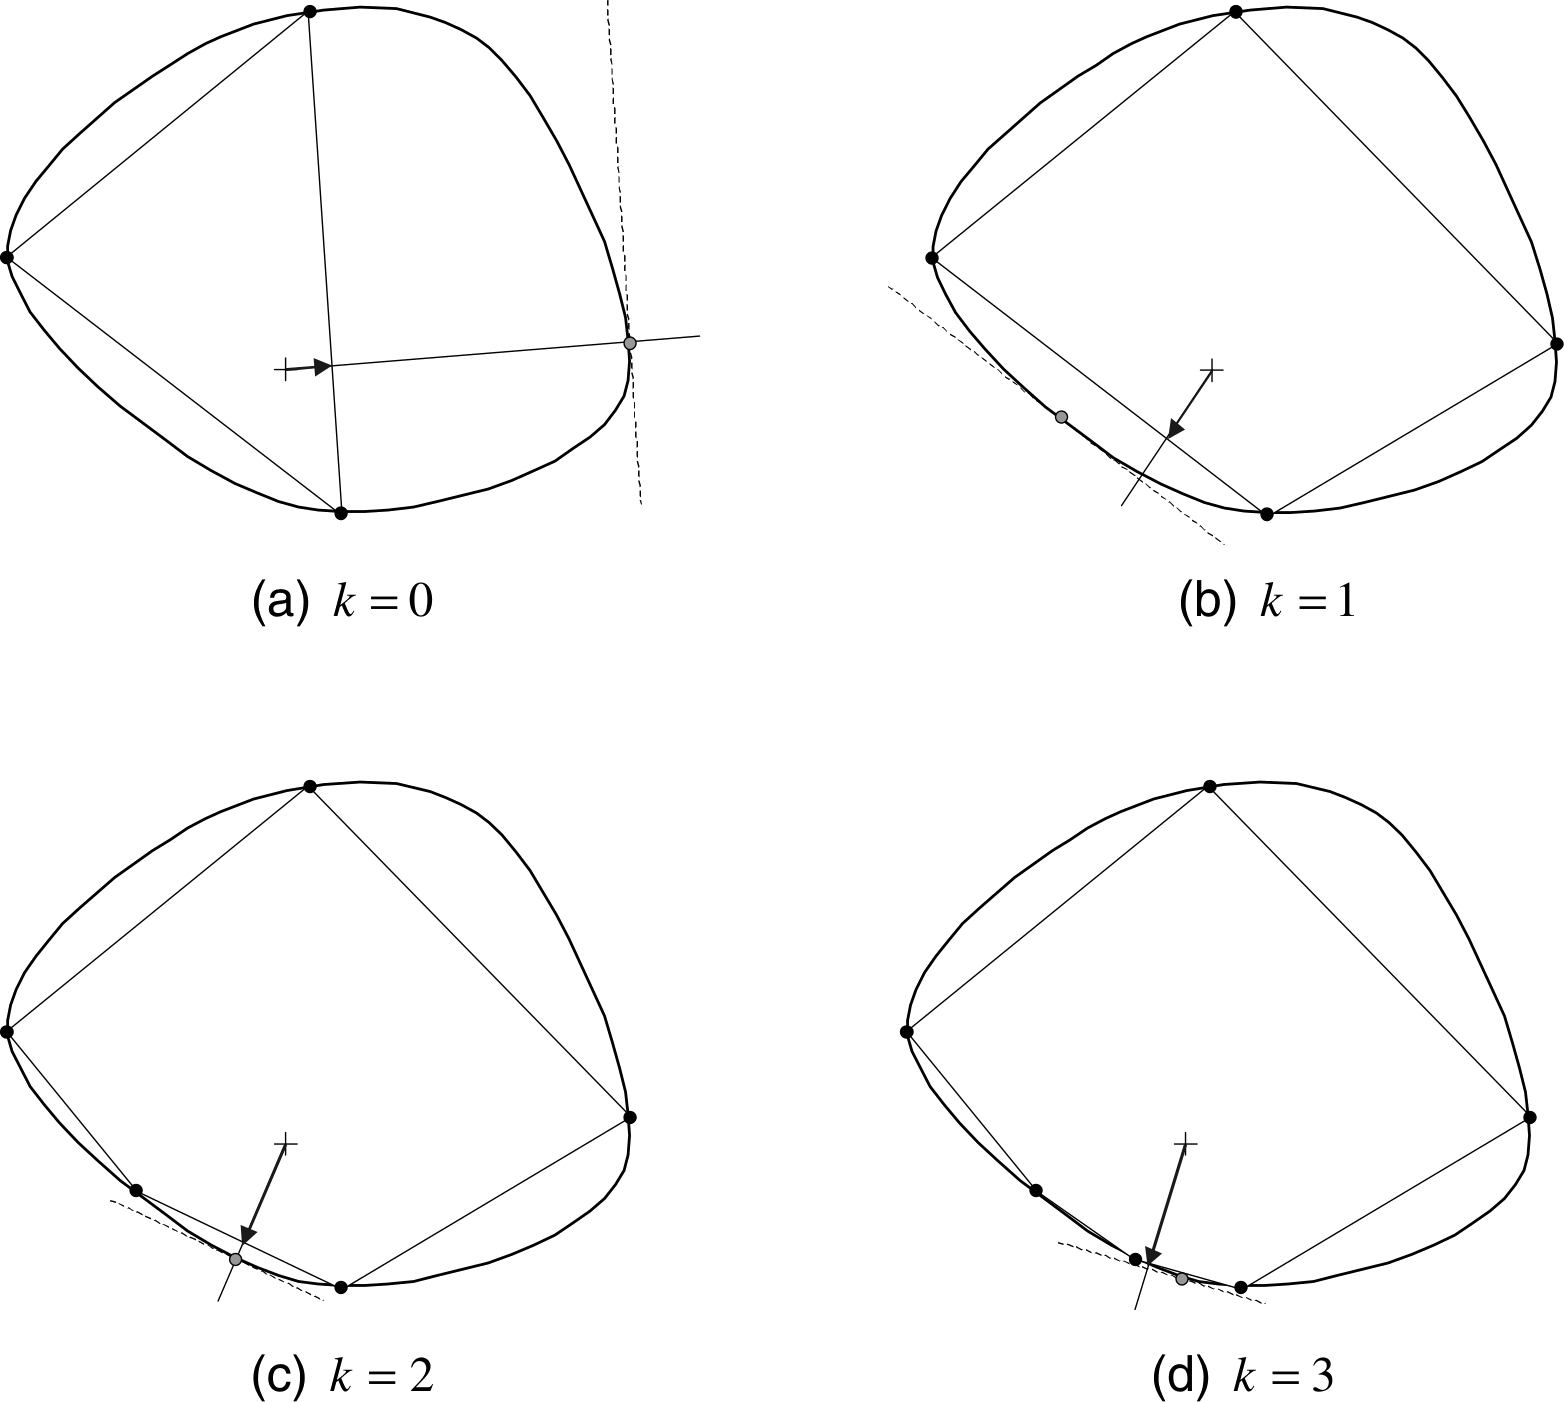
\includegraphics[width=0.7\textwidth, height=0.7\textheight, keepaspectratio]{epa.jpg}
    \caption{Uma sequência de iterações do algoritmo de expansão de politopos. Uma seta indica o vetor mais curto $\vec p$. Um ponto aberto indica o novo vértice $\vec w$. Fonte: Adaptado de~\cite{bergen2001proximity}}
    \label{fig:epa}
  \end{figure}
\end{frame}
 
% ── Slide 5: Cálculo dos pontos de contato ──────────────────
\begin{frame}{Cálculo dos Pontos de Contato}
  Após obter $\hat{n}$ e $\delta$ (via SAT+MTV ou EPA), identificam-se
  as arestas e vértices envolvidos por um \textbf{método adaptado de
  recorte}:
 
  \begin{enumerate}
    \item Para cada objeto, selecionar o \textbf{vértice mais distante}
          ao longo de $\hat{n}$; verificar os dois adjacentes e escolher
          a aresta que faz o maior ângulo com $\hat{n}$
    \item A aresta \textbf{mais perpendicular} a $\hat{n}$ torna-se a
          \textbf{aresta de referência}; a outra é a
          \textbf{aresta incidente}
    \item Vértices da aresta de referência + vértice incidente com maior
          produto escalar com $-\hat{n}$ formam o manifold
  \end{enumerate}
 
  % \begin{columns}[T]
  %   \column{0.48\textwidth}
  %     % Inserir figura das arestas envolvidas (collision-manifold-2.svg)
  %     \begin{center}
  %       \fbox{\parbox{0.88\linewidth}{\centering\vspace{2.2cm}
  %         \textit{[figura: arestas envolvidas]}
  %         \vspace{2.2cm}}}
  %     \end{center}
  %   \column{0.48\textwidth}
  %     % Inserir figura referência/incidente (collision-manifold-3.svg)
  %     \begin{center}
  %       \fbox{\parbox{0.88\linewidth}{\centering\vspace{2.2cm}
  %         \textit{[figura: aresta ref.\ e incidente]}
  %         \vspace{2.2cm}}}
  %     \end{center}
  % \end{columns}
\end{frame}

\begin{frame}
  \begin{figure}[htb]
      \centering
      \begin{minipage}{0.45\textwidth}
          \centering
      \includesvg[width=\textwidth]{collision-manifold-2}
      \caption{Cenário de colisão, arestas envolvidas em destaque. Fonte: Adaptado de~\cite{collision_manifolds_2017}.}
      \label{fig:collision-manifold-1}
      \end{minipage}
      \hfill
      \begin{minipage}{0.45\textwidth}
          \centering
      \includesvg[width=\textwidth]{collision-manifold-3}
      \caption{Aresta de referência em vermelho e aresta incidente em azul. Fonte: Adaptado de~\cite{collision_manifolds_2017}.}
      \label{fig:collision-manifold-2}
      \end{minipage}
      % \caption{Figuras lado a lado}
  \end{figure}
\end{frame}
 
% ── Slide 6: Processo de separação ──────────────────────────
\begin{frame}{Processo de Separação — Jakobsen}
  Correção total: $\vec{c} = d \cdot \hat{n}$,\;
  distribuída pelas massas inversas:
  \[
    \vec{c}_A = -\frac{w_B}{w_A+w_B}\,\vec{c},\qquad
    \vec{c}_B = +\frac{w_A}{w_A+w_B}\,\vec{c}
  \]

  \begin{itemize}
    \item Vértice-Vértice
    \item Vértice-Aresta
    \item Aresta-Aresta
  \end{itemize}
\end{frame}

\begin{frame}{Caso Vértice-Aresta}
  \begin{columns}
    \column{0.50\textwidth}
      Considere um vértice $p \in A$ e uma aresta $\overline{rs} \in B$, definida pelos vértices $r$ e $s$. Seja $w$ um ponto na aresta $\overline{rs}$, correspondente à projeção ortogonal de $p$ sobre a aresta:
      $$
      \alpha = \frac{(p - r) \cdot (s - r)}{\|s - r\|^2}, \quad \alpha \in [0,1]
      $$
    
      $$
      w = r + \alpha (s - r)
      $$
      O objetivo é deslocar $p$ e $w$ para o ponto de contato $w'$, tal que:
      $$
      w' = w + \vec c_B = p + \vec c_A
      $$
      
    \column{0.50\textwidth}
      \begin{figure}[htb]
        \centering
        \includesvg[width=0.8\textwidth]{processo-separacao}
        % \caption{Caso colisão vértice-aresta. Correção das posição para configuração válida. O vértice mais próximo de $w$ sofre maior deslocamento, preservando a coerência geométrica da aresta. Fonte: Adaptado de~\cite{jakobsen2001advanced}.}
        % \label{fig:processo-separacao}
      \end{figure}
  \end{columns}
\end{frame}

\begin{frame}
  \begin{columns}
    \column{0.5\textwidth}
      As correções aplicadas a $p$, $r$ e $s$ são:
      $$
      p' = p + \vec c_A
      $$
      $$
      r' = r + (1 - \alpha)\vec c_B, \quad
      s' = s + \alpha \vec c_B
      $$

    \column{0.50\textwidth}
      \begin{figure}[htb]
        \centering
        \includesvg[width=0.8\textwidth]{processo-separacao}
        % \caption{Caso colisão vértice-aresta. Correção das posição para configuração válida. O vértice mais próximo de $w$ sofre maior deslocamento, preservando a coerência geométrica da aresta. Fonte: Adaptado de~\cite{jakobsen2001advanced}.}
        % \label{fig:processo-separacao}
      \end{figure}
  \end{columns}

  \begin{block}{}
    A correção $c_B$ deve ser distribuída entre os vértices $r$ e $s$ da aresta de forma ponderada pelo parâmetro $\alpha$, de modo que o vértice mais próximo de $w$ receba maior fração do deslocamento.
  \end{block}
\end{frame}

% ============================================================
\section{Otimizações}
% ============================================================
 
% ── Slide 1: Problema — complexidade quadrática ──────────────
\begin{frame}{Otimizações — O Problema}
  \begin{block}{Complexidade ingênua}
    Com $n$ objetos, o número de pares a testar é:
    \[
      \frac{n(n-1)}{2} = O(n^2)
    \]
    Mesmo para valores moderados de $n$, esse custo torna-se
    impraticável em tempo real.
  \end{block}
\end{frame}

\begin{frame}
    \textbf{Solução:} separar a detecção em duas fases:
      \begin{enumerate}
        \item \textbf{Filtragem (\textit{Broad Phase})} — descartar
              rapidamente pares impossíveis com testes baratos e
              conservadores
        \item \textbf{Refinamento (\textit{Narrow Phase})} — aplicar
              SAT / GJK / EPA apenas nos pares candidatos restantes
      \end{enumerate}
      \vspace{0.2cm}
      A premissa fundamental: objetos só podem colidir se estiverem
      \textbf{suficientemente próximos}.

      \begin{alertblock}{Redução esperada}
        Em cenários bem comportados, a filtragem reduz a complexidade
        para $O(n)$ ou $O(n \log n)$, embora no pior caso (todos
        concentrados em poucas células) possa regredir a $O(n^2)$.
      \end{alertblock}
\end{frame}
 
% ── Slide 2: Objetos delimitadores ──────────────────────────
\begin{frame}{Objetos Delimitadores}
  Substituem a geometria original por formas mais simples para
    testes rápidos de sobreposição. Propriedade fundamental:
    \begin{itemize}
    \item Se os delimitadores \textbf{não} se intersectam
            $\Rightarrow$ os objetos \textbf{definitivamente não}
            colidem
    \item Se se intersectam $\Rightarrow$ \textit{possível} colisão
            (falso positivo admissível)
    \end{itemize}

    \begin{figure}[htb]
      \centering
      \includesvg[width=\linewidth]{bounding_volumes}
      \caption{Da esquerda para direita esfera delimitadora, caixa delimitadora alinhada aos eixos, caixa delimitadora orientada, K-DOP e fecho convexo. Fonte: Autor.}
      \label{fig:formas-fecho-convexo}
    \end{figure}
\end{frame}
 
% ── Slide 3: Grade uniforme — estrutura ─────────────────────
\begin{frame}{Filtragem com Grade Uniforme}
  \begin{columns}
    \column{0.5\textwidth}
      O espaço é subdividido em células de tamanho fixo $C$. Cada
      objeto é associado às células interceptadas pela sua AABB:
      \[
      i = \left\lfloor \frac{x}{C} \right\rfloor, \qquad
      j = \left\lfloor \frac{y}{C} \right\rfloor
      \]
      Chave linear da célula:
      \[
      Key_{\text{cell}} = i + j \times n_{\text{col}}
      \]
      Os pares $(Key_{\text{cell}},\, Index_{\text{obj}})$ são
      armazenados em um array e \textbf{ordenados} pela chave.
      Objetos na mesma célula ficam contíguos — favorece localidade
      de cache.
  
      \column{0.5\textwidth}
        \begin{figure}[htb]
          \centering
          \includesvg[width=0.7\textwidth, height=0.7\textheight, keepaspectratio]{uniform-grid}
          % \caption{Fonte: Autor.}
          % \caption{Divisão espacial em grade uniforme}
          \label{fig:grade-uniforme}
        \end{figure}

    \end{columns}
\end{frame}
 
% ── Slide 4: Grade uniforme — deduplicação e parâmetros ─────
\begin{frame}{Filtragem — Deduplicação e Escolha de $C$}
  \begin{block}{}
    Dois objetos são \textbf{candidatos} somente se compartilharem ao menos uma célula.
  \end{block}

  \textbf{Eliminação de duplicatas} ao percorrer o array ordenado:
  \begin{enumerate}
    \item Par $(A,B)$ testado por ordem — nunca repetir $(B,A)$
    \item Objeto grande interceptando múltiplas células pode gerar
          o mesmo par em células distintas — testar uma única vez
  \end{enumerate}

  \textbf{Escolha do tamanho de célula $C$:}
  \begin{itemize}
    \item Idealmente cada objeto ocupa $\approx$ 1 célula
          (máx.\ 4 em 2D)
    \item $C$ pequeno demais: custo de atualização elevado
    \item $C$ grande demais: muitos objetos por célula,
          filtragem ineficaz
    \item Grande variação de escala: considerar abordagens
          hierárquicas
  \end{itemize}
\end{frame}

\begin{frame}
    \begin{block}{Estratégia de reconstrução}
        A grade é \textbf{reconstruída a cada passo de tempo} a
        partir de um array linear com contador zerado. Trade-off
        deliberado: simplicidade e previsibilidade em vez de
        atualizações incrementais.
        \end{block}
        \vspace{0.3cm}
        \begin{exampleblock}{Fase de refinamento (Narrow Phase)}
        Após a filtragem, os pares candidatos passam ao
        refinamento via \textbf{SAT} ou \textbf{GJK+EPA} para
        confirmação precisa da colisão.
    \end{exampleblock}
\end{frame}

% ============================================================
\section{Resultados}
% ============================================================
 
% ── Slide 1: Metodologia ────────────────────────────────────
\begin{frame}{Metodologia de Testes}
  Quatro configurações avaliadas, variando o número de objetos
  de 100 a 1000 (incrementos de 100), com 180 quadros por configuração:
 
  \vspace{0.3cm}
  \begin{enumerate}
    \item SAT \textbf{sem} fase de filtragem
    \item SAT \textbf{com} grade uniforme na filtragem
    \item GJK/EPA \textbf{sem} fase de filtragem
    \item GJK/EPA \textbf{com} grade uniforme na filtragem
  \end{enumerate}
 
  \vspace{0.3cm}
  \begin{itemize}
    \item Testes executados \textbf{sem visualização} — isola o custo
          computacional da detecção de colisão
    \item Distribuição inicial por \textit{Poisson Disk Sampling}
          — amostras uniformes com distância mínima garantida
    \item Semente pseudoaleatória fixa para reprodutibilidade
    \item Métricas: tempo médio de execução, número de testes de
          colisão e tempo por etapa da simulação
  \end{itemize}
\end{frame}
 
% ── Slide 2: Impacto da filtragem ───────────────────────────
\begin{frame}{Impacto da Filtragem — Número de Testes de Colisão}
  \begin{center}
    % Inserir figura comparativo-testes-colisao.png
    \fbox{\parbox{0.88\linewidth}{\centering\vspace{5.5cm}
      \textit{[figura: número médio de testes de colisão (escala log)]}
      \vspace{5.5cm}}}
  \end{center}
 
  \vspace{0.2cm}
  A grade uniforme reduz drasticamente o número de pares avaliados.
  Resultados em \textbf{escala logarítmica} pela diferença de ordens
  de grandeza entre os cenários com e sem filtragem.
\end{frame}
 
% ── Slide 3: Profiling SAT ──────────────────────────────────
\begin{frame}{Tempo por Etapa — Modo SAT}
  \begin{center}
    % Inserir figura profiling-sat.png
    \fbox{\parbox{0.88\linewidth}{\centering\vspace{5.8cm}
      \textit{[figura: tempo relativo por etapa — modo SAT]}
      \vspace{5.8cm}}}
  \end{center}
 
  \vspace{0.2cm}
  A etapa de \textbf{relaxamento} domina o custo total em todos os
  cenários, seguida por filtragem e refinamento.
\end{frame}
 
% ── Slide 4: Profiling GJK ──────────────────────────────────
\begin{frame}{Tempo por Etapa — Modo GJK/EPA}
  \begin{center}
    % Inserir figura profiling-gjk.png
    \fbox{\parbox{0.88\linewidth}{\centering\vspace{5.8cm}
      \textit{[figura: tempo relativo por etapa — modo GJK/EPA]}
      \vspace{5.8cm}}}
  \end{center}
 
  \vspace{0.2cm}
  O GJK/EPA apresenta \textbf{maior custo} na fase de refinamento
  em relação ao SAT. O relaxamento permanece dominante.
\end{frame}
 
% ── Slide 5: Gargalo do relaxamento ─────────────────────────
\begin{frame}{Análise: Gargalo do Relaxamento}
  \begin{block}{Por que o relaxamento domina?}
    O método de Jakobsen exige \textbf{múltiplas iterações} (5 neste
    trabalho) para convergir. O custo cresce proporcionalmente ao
    número de restrições e passos de relaxamento.
  \end{block}
 
  \vspace{0.3cm}
  \textbf{Caminhos para otimização identificados:}
  \begin{itemize}
    \item Reduzir o número de iterações de relaxamento
    \item Substituir a grade uniforme por estruturas hierárquicas
          (BVH, \textit{Quadtree}) na filtragem
    \item Paralelizar etapas via \textbf{multi-thread} (Web Workers)
    \item Delegar cálculos intensivos à GPU via \textbf{WebGPU}
  \end{itemize}
\end{frame}
 
% ── Slide 6: Comparação com Planck.js ───────────────────────
\begin{frame}{Comparação com \textit{Planck.js} — Tempo de Execução}
  \begin{center}
    % Inserir figura comparativo-tempo-execução.png
    \fbox{\parbox{0.88\linewidth}{\centering\vspace{5.5cm}
      \textit{[figura: tempo médio de execução — nossa impl.\ vs Planck.js]}
      \vspace{5.5cm}}}
  \end{center}
 
  \vspace{0.2cm}
  A \textit{Planck.js} apresenta desempenho superior em todos os
  cenários avaliados.
\end{frame}
 
% ── Slide 7: Análise da comparação ──────────────────────────
\begin{frame}{Por que \textit{Planck.js} é mais rápida?}
  \begin{block}{Nossa implementação}
    \begin{itemize}
      \item Resolução por \textbf{relaxamento iterativo} (Jakobsen)
            — múltiplas iterações por passo de tempo
      \item Filtragem via \textbf{grade uniforme} — simples, mas menos
            adaptativa a variações de escala
    \end{itemize}
  \end{block}
 
  \vspace{0.3cm}
  \begin{block}{\textit{Planck.js} (baseada no Box2D)}
    \begin{itemize}
      \item Resolução por \textbf{impulsos} — colisões resolvidas
            diretamente no nível dos corpos rígidos, mais eficiente
            por passo de tempo
      \item Filtragem com \textbf{árvore dinâmica de AABB}
            — hierárquica, mais adaptada a cenários heterogêneos
    \end{itemize}
  \end{block}
 
  \begin{alertblock}{}
    O objetivo deste trabalho não é superar a \textit{Planck.js}, mas
    oferecer uma implementação \textbf{didática, modular e aberta},
    que evidencie cada etapa do pipeline de simulação física.
  \end{alertblock}
\end{frame}
 
% ============================================================
\section{Conclusão}
% ============================================================
 
\begin{frame}{Conclusões}
  \begin{itemize}
    \item Foi implementado um motor de animação física funcional
          inteiramente em JavaScript/WebGL
    \item A integração de Verlet mostrou-se adequada e estável
          para simulações em tempo real no navegador
    \item O método de Jakobsen por relaxamento de restrições
          proporcionou comportamento visualmente plausível
    \item Desempenho satisfatório para aplicações interativas
          típicas ($\leq 300$ corpos a 60\,FPS)
    \item Código aberto e bem documentado — adequado para uso didático
  \end{itemize}
\end{frame}
 
% ── ── ── ── ── ── ── ── ── ── ── ── ── ── ── ── ── ── ── ──
\begin{frame}{Trabalhos Futuros}
  \begin{enumerate}
    \item Implementar grade espacial / BVH para fase ampla mais eficiente
    \item Adicionar suporte a articulações e restrições angulares
    \item Explorar WebGPU para cálculos físicos em GPU
    \item Estender para 3D com suporte a quatérnios
  \end{enumerate}
\end{frame}

% ── ── ── ── ── ── ── ── ── ── ── ── ── ── ── ── ── ── ── ──
\begin{frame}{Referências}
  \footnotesize
  \begin{thebibliography}{9}
    \bibitem{azevedo2003}
      E.~Azevedo, A.~Conci.
      \textit{Computação Gráfica}.
      Campus, 2003.
 
    \bibitem{jakobsen2001advanced}
      T.~Jakobsen.
      Advanced character physics.
      \textit{Game Developer Conference}, 2001.
 
    \bibitem{ericson2004real}
      C.~Ericson.
      \textit{Real-Time Collision Detection}.
      Morgan Kaufmann, 2004.
 
    \bibitem{box2d_physics}
      E.~Catto.
      \textit{Box2D — A 2D Physics Engine for Games}.
      \url{https://box2d.org/}, 2007.
 
    \bibitem{matterjs}
      L.~Brewer.
      \textit{Matter.js — 2D Physics Engine for the Web}.
      \url{https://brm.io/matter-js/}, 2014.
  \end{thebibliography}
\end{frame}

% ── Slide final ─────────────────────────────────────────────
\begin{frame}[plain]
  \vfill
  \begin{center}
    {\Large\textbf{Obrigado!}}\\[1cm]
    Dúvidas e discussão\\[0.8cm]
    \texttt{diegovsm@ic.ufjr.br}
  \end{center}
  \vfill
\end{frame}

\end{document}